%\usepackage{multicol}
\usepackage{calc}
\usepackage{ifthen}
\usepackage[landscape]{geometry}


% Times for rm and math | Helvetica for ss | Courier for tt
\usepackage{mathptmx} % rm & math
\usepackage[scaled=0.90]{helvet} % ss
\usepackage{courier} % tt
\normalfont
\usepackage[T1]{fontenc}
\usepackage{graphicx}
\usepackage{color}

%% Palatino for rm and math | Helvetica for ss | Courier for tt
%\usepackage{mathpazo} % math & rm
%\linespread{1.05}        % Palatino needs more leading (space between lines)
%\usepackage[scaled]{helvet} % ss
%\usepackage{courier} % tt
%\normalfont
%\usepackage[T1]{fontenc}

%% Euler for math | Palatino for rm | Helvetica for ss | Courier for tt
%\renewcommand{\rmdefault}{ppl} % rm
%\linespread{1.05}        % Palatino needs more leading
%\usepackage[scaled]{helvet} % ss
%\usepackage{courier} % tt
%\usepackage{euler} % math
%%\usepackage{eulervm} % a better implementation of the euler package (not in gwTeX)
%\normalfont
%\usepackage[T1]{fontenc}



% To make this come out properly in landscape mode, do one of the following
% 1.
%  pdflatex latexsheet.tex
%
% 2.
%  latex latexsheet.tex
%  dvips -P pdf  -t landscape latexsheet.dvi
%  ps2pdf latexsheet.ps


% If you're reading this, be prepared for confusion.  Making this was
% a learning experience for me, and it shows.  Much of the placement
% was hacked in; if you make it better, let me know...


% 2008-04
% Changed page margin code to use the geometry package. Also added code for
% conditional page margins, depending on paper size. Thanks to Uwe Ziegenhagen
% for the suggestions.

% 2006-08
% Made changes based on suggestions from Gene Cooperman. <gene at ccs.neu.edu>


% To Do:
% \listoffigures \listoftables
% \setcounter{secnumdepth}{0}


% This sets page margins to .5 inch if using letter paper, and to 1cm
% if using A4 paper. (This probably isn't strictly necessary.)
% If using another size paper, use default 1cm margins.
\ifthenelse{\lengthtest { \paperwidth = 11in}}
	{ \geometry{top=.5in,left=.5in,right=.5in,bottom=.5in} }
	{\ifthenelse{ \lengthtest{ \paperwidth = 297mm}}
		{\geometry{top=1cm,left=1cm,right=1cm,bottom=1cm} }
		{\geometry{top=1cm,left=1cm,right=1cm,bottom=1cm} }
	}

% Turn off header and footer
\pagestyle{empty}
 

% Redefine section commands to use less space
\makeatletter
\renewcommand{\section}{\@startsection{section}{1}{0mm}%
                                {-1ex plus -.5ex minus -.2ex}%
                                {0.5ex plus .2ex}%x
                                {\normalfont\large\bfseries}}
\renewcommand{\subsection}{\@startsection{subsection}{2}{0mm}%
                                {-1explus -.5ex minus -.2ex}%
                                {0.5ex plus .2ex}%
                                {\normalfont\normalsize\bfseries}}
\renewcommand{\subsubsection}{\@startsection{subsubsection}{3}{0mm}%
                                {-1ex plus -.5ex minus -.2ex}%
                                {1ex plus .2ex}%
                                {\normalfont\small\bfseries}}
\makeatother

% Define BibTeX command
\def\BibTeX{{\rm B\kern-.05em{\sc i\kern-.025em b}\kern-.08em
    T\kern-.1667em\lower.7ex\hbox{E}\kern-.125emX}}

% Don't print section numbers
\setcounter{secnumdepth}{0}


\setlength{\parindent}{0pt}
\setlength{\parskip}{0pt plus 0.5ex}


% -----------------------------------------------------------------------

\begin{document}

\raggedright
\footnotesize
%\begin{multicols}{2}


% multicol parameters
% These lengths are set only within the two main columns
%\setlength{\columnseprule}{0.25pt}
%\setlength{\premulticols}{1pt}
%\setlength{\postmulticols}{1pt}
%\setlength{\multicolsep}{1pt}
%\setlength{\columnsep}{2pt}

\begin{center}
     \Large{\textbf{Score-P Cheat Sheet}} \\
\end{center}

\begin{minipage}[c]{.72\columnwidth}
\subsection{General Workflow Loop}

\vspace{1em}
\begin{itemize}
\itemsep0.1em
\item \textbf{Preparation}: instrument target application and set up measurement environment
\item \textbf{Measurement}: run application with measurement infrastructure enabled
\item \textbf{Analysis}: analyse generated performance data
\item \textbf{Examination}: find possible cause of performance anomalies in the code
\item \textbf{Optimization}: apply optimizations to eliminate bottleneck
\item \textbf{Repeat}: apply analysis workflow loop until acceptable performance achieved
\end{itemize}
\end{minipage}
\hspace{.05\columnwidth}
\begin{minipage}{.15\columnwidth}
%\begin{figure}
\centering
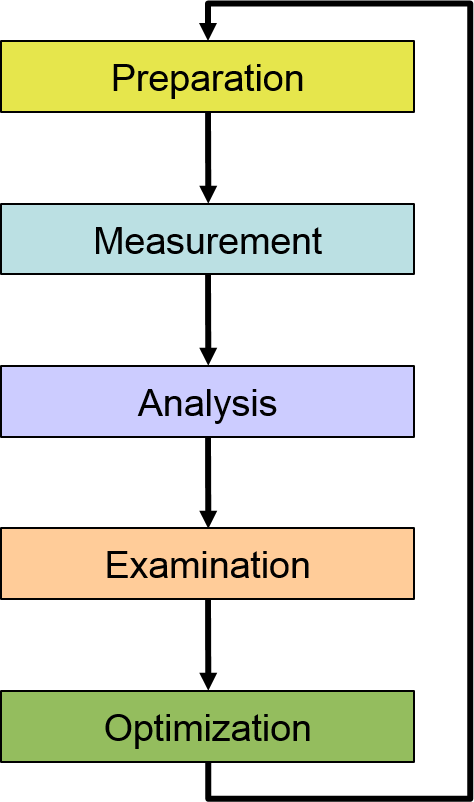
\includegraphics[width=\textwidth]{Workflow}
%\caption{The intended workflow loop}
%\end{figure}
\end{minipage}

\subsection{Performance Analysis Procedure}
  
\begin{itemize}
\itemsep0.1em
\item  Create a profile with full instrumentation
\item  Compare runtime to uninstrumented run to determine overhead
\item  (Incrementally) create filter file using hints from the
      \texttt{scorep-score} tool
\item  Create an optimized profile with filter applied
\item  Investigate profile with CUBE
\item  For in-depth analysis, generate a trace \textbf{with filter applied}
      and examine it using Scalasca and than Vampir
\end{itemize}


\subsection{Application Instrumentation}
\begin{itemize}
\itemsep0.1em
\item Prefix all compile/link commands with \texttt{scorep}\\
\item Compile as usual\\
\item Advanced instrumentation options available to further adjust the measurement configuration
\end{itemize}
\subsection{Application Measurement}
Set Score-P environment variables\\[1ex]
\begin{tabular}{@{}l@{ }l@{ }}
\texttt{SCOREP\_EXPERIMENT\_DIRECTORY} & Name of the experiment directory\\
\texttt{SCOREP\_ENABLE\_PROFILING} & Enable generation of profiles (default)\\
\texttt{SCOREP\_ENABLE\_TRACING} & Enable the generation of traces\\
\texttt{SCOREP\_TOTAL\_MEMORY} & Total memory in bytes used for the measurement system per process\\
\texttt{SCOREP\_FILTERING\_FILE} & Name of file containing filter rules\\
\end{tabular}\\[1ex]
... and many more (see manual or run \texttt{scorep-info config-vars ---full})\\

% Push down the right column below title on the left column
\setlength{\topskip}{3em}
Run application as usual:\\
\texttt{ \% export SCOREP\_ENABLE\_TRACING=false}\\
\texttt{ \% export SCOREP\_ENABLE\_PROFILING=true}\\
\texttt{ \% export SCOREP\_EXPERIMENT\_DIRECTORY=scorep\_run}\\
\texttt{ \% export OMP\_NUM\_THREADS=4}\\
\texttt{ \% mpirun -np 4 ./binary\_scorep}\\

\vspace{1em}

\subsection{Profile Examination with CUBE and Filter File Creation}
Analyze profile with CUBE\\
\texttt{ \% cube scorep\_run/profile.cubex}\\
Create filter file with hints from \texttt{scorep-score}\\
\texttt{ \% scorep-score -r scorep\_run/profile.cubex}\\
\texttt{ \% scorep-score -r -f ./scorep.filt scorep\_run/profile.cubex}\\
Create profile with filter applied\\
\texttt{ \% export SCOREP\_EXPERIMENT\_DIRECTORY=scorep\_run\_filter}\\
\texttt{ \% export SCOREP\_FILTERING\_FILE=./scorep.filt}\\
\texttt{ \% mpirun -np 4 ./binary\_scorep}\\


\subsection{Automatic Trace Analysis with Scalasca}
Run the application using Scalasca with trace collection and analysis\\
\texttt{ \% export SCOREP\_EXPERIMENT\_DIRECTORY=scorep\_run\_trace}\\
\texttt{ \% export OMP\_NUM\_THREADS=4}\\
\texttt{ \% export SCOREP\_TOTAL\_MEMORY=25M}\\
\texttt{ \% scan -f ./scorep.filt -t mpirun -np 4 ./binary\_scorep}\\
Produces and examine trace analysis report\\
\texttt{ \% square scorep\_run\_trace}\\

\subsection{Interactive Performance Analysis with Vampir}
\textbf{Open small traces direclty in Vampir}\\
\texttt{ \% vampir scorep\_run\_trace/traces.otf2}\\[2ex]

\textbf{Open large traces using VampirServer}\\
1. Launch analysis server on remote machine\\
\texttt{ \% ssh remote-machine}\\
\texttt{ \% vampirserver start -n 4 }\\
\texttt{ Running 4 analysis processes... (abort with vampirserver stop 17950)}\\
\texttt{ VampirServer <17950> listens on: \textcolor{red}{node123:30085}}\\[2ex]

2. Open SSH tunnel to connect remote VampirServer with GUI on your local machine\\
\texttt{ \% ssh -L30000:\textcolor{red}{node123:30085} mymachine}\\[2ex]

3. Open Vampir and connect to VampirServer (listening on localhost:30000 via SSH tunnel)\\
\texttt{ \% vampir localhost:30000:scorep\_run\_trace/traces.otf2}\\[2ex]

4. Shutdown VampirServer on remote machine when finished\\
\texttt{ \% ssh remote-machine}\\
\texttt{ \% vampirserver stop}



\vfill
\pagebreak

\section{PAPI Hardware Performance Counters}
\verb|VT_METRICS=PAPI_FP_OPS:PAPI_L2_TCM:!CPU_TEMP1|\\
\texttt{CPU\_TEMP1} is provided by the lm-sensors component.\\ 
See \texttt{papi\_avail} and \texttt{papi\_native\_avail} for available counter.
\begin{scriptsize}
\begin{verbatim}
PAPI_L[1|2|3]_[D|I|T]C[M|H|A|R|W]    
              Level 1/2/3 data/instruction/total cache 
              misses/hits/accesses/reads/writes
PAPI_L[1|2|3]_[LD|ST]M    
              Level 1/2/3 load/store misses                       
PAPI_CA_SNP   Requests for a snoop                                
PAPI_CA_SHR   Req. for excl. access to shared cache line  
PAPI_CA_CLN   Req. for excl. access to clean cache line   
PAPI_CA_INV   Requests for cache line invalidation                
PAPI_CA_ITV   Requests for cache line intervention                
PAPI_BRU_IDL  Cycles branch units are idle                        
PAPI_FXU_IDL  Cycles integer units are idle                       
PAPI_FPU_IDL  Cycles floating point units are idle                
PAPI_LSU_IDL  Cycles load/store units are idle                    
PAPI_TLB_DM   Data translation lookaside buffer misses            
PAPI_TLB_IM   Instruction transl. lookaside buffer misses     
PAPI_TLB_TL   Total translation lookaside buffer misses           
PAPI_BTAC_M   Branch target address cache misses                  
PAPI_PRF_DM   Data prefetch cache misses                          
PAPI_TLB_SD   Translation lookaside buffer shootdowns             
PAPI_CSR_FAL  Failed store conditional instructions               
PAPI_CSR_SUC  Successful store conditional instructions           
PAPI_CSR_TOT  Total store conditional instructions                
PAPI_MEM_SCY  Cycles Stalled Waiting for memory accesses          
PAPI_MEM_RCY  Cycles Stalled Waiting for memory Reads             
PAPI_MEM_WCY  Cycles Stalled Waiting for memory writes            
PAPI_STL_ICY  Cycles with no instruction issue                    
PAPI_FUL_ICY  Cycles with maximum instruction issue               
PAPI_STL_CCY  Cycles with no instructions completed               
PAPI_FUL_CCY  Cycles with maximum instructions completed          
PAPI_BR_UCN   Unconditional branch instructions                   
PAPI_BR_CN    Conditional branch instructions                     
PAPI_BR_TKN   Conditional branch instructions taken               
PAPI_BR_NTK   Conditional branch instructions not taken           
PAPI_BR_MSP   Conditional branch inst. mispredicted        
PAPI_BR_PRC   Cond. branch inst. correctly predicted 
PAPI_FMA_INS  FMA instructions completed                          
PAPI_TOT_IIS  Instructions issued                                 
PAPI_TOT_INS  Instructions completed                              
PAPI_INT_INS  Integer instructions                                
PAPI_FP_INS   Floating point instructions                         
PAPI_LD_INS   Load instructions                                   
PAPI_SR_INS   Store instructions                                  
PAPI_BR_INS   Branch instructions                                 
PAPI_VEC_INS  Vector/SIMD instructions                            
PAPI_LST_INS  Load/store instructions completed                   
PAPI_SYC_INS  Synchronization instructions completed              
PAPI_FML_INS  Floating point multiply instructions                
PAPI_FAD_INS  Floating point add instructions                     
PAPI_FDV_INS  Floating point divide instructions                  
PAPI_FSQ_INS  Floating point square root instructions             
PAPI_FNV_INS  Floating point inverse instructions                 
PAPI_RES_STL  Cycles stalled on any resource    
PAPI_FP_STAL  Cycles the FP unit(s) are stalled 
PAPI_FP_OPS   Floating point operations         
PAPI_TOT_CYC  Total cycles                      
PAPI_HW_INT   Hardware interrupts               
\end{verbatim} 
\end{scriptsize}

\vfill

\section{Resource Usage Counters}
The Unix system call \texttt{getrusage} provides information about consumed  resources and operating system events.\\
\verb|VT_RUSAGE=ru_stime:ru_majflt|\\
The resource usage counters are not recorded at every event. Set intervall in ms:\\
\texttt{export VT\_RUSAGE\_INTV=100} (most OS support min. of 10ms )\\
Counters are per process, not per thread.\\
\begin{tabular}{@{}l@{}l@{ }c@{ }l@{}}
\textbf{Name}          &  \textbf{Unit}  & \textbf{Linux} & \textbf{Description}  \\
\texttt{ru\_utime}     &  ms             & x         & Total amount of user time used.  \\
\texttt{ru\_stime}     &  ms             & x         & Total amount of system time used.  \\
\texttt{ru\_maxrss}    &  kB             &           & Maximum resident set size. \\
\texttt{ru\_ixrss}     &  kB/s           &           & Integral shared memory size (text segment). \\
\texttt{ru\_idrss}     &  kB/s           &           & Integral data segment memory used over runtime. \\
\texttt{ru\_isrss}     &  kB/s           &           & Integral stack memory used over the runtime. \\
\texttt{ru\_minflt}    &  \#             & x         & Number of soft page faults. \\
\texttt{ru\_majflt}    &  \#             & x         & Number of hard page faults. \\
\texttt{ru\_nswap}     &  \#             &           & \# times process was swapped out of phys. mem. \\
\texttt{ru\_inblock}   &  \#             &           & Number of input operations via the file system. \\
\texttt{ru\_oublock}   &  \#             &           & Number of output operations via the file system. \\
\texttt{ru\_msgsnd}    &  \#             &           & Number of IPC messages sent. \\
\texttt{ru\_msgrcv}    &  \#             &           & Number of IPC messages received. \\
\texttt{ru\_nsignals}  &  \#             &           & Number of signals delivered. \\
\texttt{ru\_nvcsw}     &  \#             & x         & Number of voluntary context switches. \\
\texttt{ru\_nivcsw}    &  \#             & x         & Number of involuntary context switches. \\
\end{tabular}\\
\vspace*{32em}

%\end{multicols}
\end{document}

